\chapter{Проблема формалізації голосової інформації в системах диспетчерського контролю за рухом автотранспорту} \label{chapt1}

\section{Проблема формалізації голосової інформації в системах диспетчерського контролю за рухом автотранспорту} \label{sect1_1}

Дистрибуція — це діяльність, пов'язана з отриманням продукції, її зберіганням до моменту отримання замовлення і наступної доставки до клієнтів. Управління дистрибуцією включає в себе планування, організацію та контроль.

Інформаційні технології в управлінні дистрибуцією вже достатньо розроблені для забезпечення етапів отримання продукції та її збереження, отже зараз найбільш інтенсивно йде розвиток етапу доставки продукції до кінцевих клієнтів. Зокрема розробляються системи автоматизації побудови планових маршрутів руху автотранспорту \cite{art1}, системи керування транспортним парком (TMS) та моніторинг доставок у реальному часі.

Велику роль в управлінні дистрибуцією відіграють процеси голосової взаємодії, які зараз активно автоматизуються для підвищення ефективності, збереження ресурсів тощо. Голосова взаємодія поділяється на безпосередню та із залученням інформаційних технологій. Інформаційні технології в цьому контексті можуть слугувати лише засобом забезпечення зв’язку, що саме по собі може давати ефект, але найкращий результат можна отримати, якщо внести певні автоматизації голосової взаємодії.

\section{Сучасний етап автоматизації голосового управління в організаційно-технічних системах} \label{sect1_2}

Голосове управління уже має певну історію використання в транспортній сфері. Передові автоконцерни світу, такі як Ford Motor Company, BMW AG, Daimler AG прагнуть підвищити безпеку та комфорт водія, тому створюють можливість керування бортовою електронікою за допомогою голосу \cite{Kravchenko_2009}. Перша подібна система, що мала назву Linguatronic, була представленана інженерами Mercedes в автомобілі S-класу в 1996 році \cite{Heisterkamp_2001}. Вона реалізувала голосове управління функціями вбудованого телефону та адресної книги, радіо та CD-програвача, а також кондиціонеру. Fiat, працюючи з Microsoft, розробив систему з ініціацією водієм Blue\&Me, в якій перед початком мовної команди треба було натиснути кнопку на кермі. Інженери BMW також розробили систему з ініціацією водієм, що була інтегрована з їх системою управління бортовою електронікою iDrive. Honda, використовуючи систему розпізнання мови IBM ViaVoice, надала можливість керування GPS навігацією для голосового вказування адреси прибуття \cite{Jonsson_2009}.

Крім того, за наявності достатньо потужної системи, голосову взаємодію з водієм можна використовувати для підтримання діалогу під час руху вночі, аби не дати водію заснути \cite{Kravchenko_2012}.

Також проводилися дослідження з розробки систем мовного управління бортовим обладнанням літаків, але через високі вимоги до швидкості та якості розпізнання, особливо за наявності потужних шумів та перешкод, вони ще досі не були запроваджені \cite{Korsun_2013}.

Використання таких часткових функцій голосового управління, які підвищують комфорт водія, також повинно мати певний позитивний ефект. Проте ці функції не забезпечують оптимізації саме процесів дистрибуції.

У сучасних системах автоматизації дистрибуції, доставки і керування транспортним парком достатньо розробленим є і процес автоматизації побудови планових маршрутів руху автотранспорту \cite{art1}. Він включає в себе складові врахування топології, часових параметрів точки доставки (часові вікна доступності та час, необхідний на обслуговування точки), завантаженість автомобіля, кількісь доступного транспорту тощо. Проте проблема вчасного корегування маршруту у випадках, коли реальний стан справ перестає відповідати запланованому маршруту, викликає достатньо великі витрати часу на комунікацію. Якби ці функції реалізувалися за допомогою автоматизованої голосової взаємодії, це дало б максимальний ефект для покращення управління дистрибуцією.

\section{Автоматизація управління в системах дистрибуції} \label{sect1_3}

Для управління доставкою вантажів у дистрибуції вкрай важливим є етап моніторингу руху автомобілів у режимі реального часу. Це дозволяє аналізувати ефективність водія, а також передбачати певні небажані інциденти. Для такого моніторингу використовують GPS дані руху автомобіля\cite{Gonzalez_2013,Comendador_2012}. На жаль лише GPS треку не достатньо для однозначного розуміння стану справ. З треку тільки й видно, що водій був біля точки доставки, але не зрозуміло, чи виконана доставка, чи з якихось причин відмінена. З треку ясно, що за поточної швидкості водій відстає від плану та не встигає на наступну точку, але не зрозумілі причини відставання та чи має водій можливість надолужити втрачений час. Для отримання цієї інформації необхідна додаткова комунікація водія з диспетчером. Але дзвінок по телефону чи, ще гірше, комунікація через якийсь візуальний інтерфейс у смартфоні забирає певний час та знижує концентрацію уваги водія на дорозі, що може спричинити ДТП. Тому потрібна система, яка б дала змогу виявляти необхідну інформацію в голосових даних водія і відправляти її диспетчеру у формалізованому вигляді.

Найбільш подібна до цього система Pick-by-Voice \cite{Pick-to-Voice}. Це система, що використовується в іншій сфері управління дистрибуцією — управлінні складськими процесами. Pick-by-Voice дає змогу відбірнику по черзі отримувати голосові команди у вигляді: де, що і в якій кількості треба відібрати, а також у формі діалогу повідомляти про необхідність повторити завдання чи переходити до наступного тощо. Така система дає змогу звільнити руки та очі відбірнику і в цілому збільшити його ефективність на 35\% \cite{Baumann_2012}.

На жаль для управління транспортними доставками потрібна більш складна система, ніж наявні можливості Pick-by-Voice, адже вона повинна мати суттєво більший спектр необхідних для розпізнання команд. У передових системах управління міськими доставками вантажів (urban freight distribution) важливим параметром є часові вікна доставки \cite{Quak_2006}. Такий параметр зразу вводить цілу низку додаткової інформації, яку треба передати від водія до диспетчера — наскільки вчасно були виконані доставки, скільки часу було витрачено на кожну з них, відставання від плану внаслідок пробок або інших непередбачуваних обставин тощо. Більше того, система повинна забезпечувати взаємодію з диспетчером у режимі реального часу, а не відтворювати заданий заздалегідь перелік завдань.

Таким чином, очевидною стає необхідність упровадження системи голосової взаємодії між водієм та диспетчером для отримання необхідної інформації від водія в мовнiй формі та автоматизації управління дистрибуцією.

\section{Сучасні наробки обробки та формалізації голосової інформації} \label{sect1_4}

\subsection{Аналіз з використанням перетворення Фур'є}

ПФ використовується в багатьох областях науки, в тому числі і в мовних технологіях. В області обробки мовних сигналів ПФ розглядається як перетворення сигналу з часової в частотну область і розкладання його на частотні складові:

\begin{equation}
\label{eq:equation1}
S(\omega)=\int_{-\infty}^{+\infty}s(t)e^{-j\omega t}dt;
\end{equation}

\begin{equation}
\label{eq:equation2}
s(t)=\frac{1}{2\pi}\int_{-\infty}^{+\infty}S(\omega)e^{j\omega t}d\omega,
\end{equation}

\noindent
де $S(\omega)$ --- сигнал в частотній області; $s(t)$ --- сигнал в часовій області; $j$ --- уявна одиниця.

У завданнях цифрової обробки часто використовують дискретне перетворення Фур'є, так як мовний сигнал часто представляють в дискретному вигляді, як суму гармонійних складових:

\begin{equation}
\label{eq:equation3}
S(k)=\sum_{n=0}^{N-1}s(nT)e^{-jk\omega nT},
\end{equation}

\noindent
де $k$ --- номер гармоніки; $\omega=\frac{2\pi}{(N-1)T}$ --- частота першої гармоніки; $0<n<N$ --- дискретні відліки часу; $T$ --- період частоти дискретизації.

Побудова спектра з використанням ДПФ дозволяє компактно і наочно представити інформацію про мовний сигнал. Однак в спектральному вигляді неможливо детально аналізувати короткочасні локальні особливості, що є серйозним недоліком ДПФ \cite{Сергиенко_2002}.

\subsection{Аналіз з використанням вейвлет-перетворення}

Незважаючи на широку практичну популярність ПФ, останнім часом багато завдань в області обробки мовних сигналів реалізуються з використанням ВП. Вейвлетом (материнським вейвлетом) називається деяка функція, добре локалізована (тобто зосереджена в невеликій околиці деякої точки і різко спадна до нуля в міру віддалення від неї) як в часовій, так і в частотній області. До материнського вейвлету застосовуються дві операції: зсування (переміщення області локалізації в часі) і масштабування (розтягування або стиснення, тобто переміщення області його локалізації за частотою):

\begin{equation}
\label{eq:equation4}
\psi_{u,s}(t)=\frac{1}{\sqrt{s}}\psi(\frac{t-u}{s}),
\end{equation}

\noindent
де $u$, $s$ – параметри зсуву.

Сутність ВП полягає в розбитті сигналу на масштабовані і зсунуті по осі часу версії материнського вейвлета та у обчисленні коефіцієнтів кореляції ділянок вихідного сигналу і версій вейвлета на заданому масштабі. В результаті виходить набір коефіцієнтів, що показують, наскільки поведінка сигналу в даний момент часу схоже на поведінку вейвлета на даному масштабі, тобто вейвлет-коефіцієнти відображають близькість сигналу до вейвлету даного масштабу. Чим ближче вигляд аналізованого сигналу в околиці даного моменту часу до вигляду вейвлета, тим більше абсолютне значення має відповідний коефіцієнт.

Використання зсуву і масштабування в частотно-часової області дозволяє аналізувати мовні сигнали на різних масштабах і точно визначати положення їхніх характерних особливостей в часі. Найбільш часто зустрічаються вейвлет-функції в задачах обробки мовних сигналів: вейвлет Хаара, вейвлет Добеши, вейвлет «Мексиканська капелюх», вейвлет Марлет (комплексний базис) \cite{Майдан_2007}.

Вейвлет-перетворення має істотні переваги в порівнянні з перетворенням Фур'є. Це випливає з можливості аналізувати короткочасні локальні особливості сигналів, наприклад, короткі сплески чи провали, розриви та сходинки і т.д.

\subsection{Аналіз з використанням декомпозиції на емпіричні моди і перетворення Гільберта-Хуанга}

Відомо, що для адаптивного аналізу мовних сигналів за допомогою ВП необхідно використовувати апріорну інформацію - функцію материнського вейвлета. Питання про вибір відповідної функції вейвлета на основі характеристик аналізованого сигналу не завжди є однозначним. Для вирішення проблеми адаптивності використовується новий метод обробки, заснований на ПГХ. Основною перевагою даного методу є висока адаптивність, що виявляється в тому, що базисні функції, які використовуються при розкладанні звуку, витягуються безпосередньо з самого вихідного сигналу і дозволяють враховувати тільки йому властиві особливості.

ПГХ включає два основних етапи:

1. Розкладання сигналу на компоненти --- декомпозиція на емпіричні моди \cite{Huang_1998,Tychkov_2013}:

\begin{equation}
\label{eq:equation5}
s(t)=\sum_{i=1}^{I-1}imf_i(t)+r_I(t),
\end{equation}

\noindent
де $imf_i(t)$ --- емпіричні моди (ЕМ); $r_I(t)$ --- залишок розкладання, $i=1,2,...,I$ --- номер ЕМ.

2. Формування за отриманими ЕМ спектру Гільберта \cite{Huang_2013}:

\begin{equation}
\label{eq:equation6}
HHT(t)=\sum_{i=1}^{T}a_i^2(t)e^{q\int\omega_k(t)dt},
\end{equation}

\noindent
де $a_i(t)=\sqrt{imf_i(t)^2+IMF_i(t)^2}$ --- модуль миттєвого значення амплітуди сигналу кожної ЕМ; $imf_i(t)$ --- ЕМ сигналу; $IMF_i(t)=\frac{1}{\pi}\int\frac{imf_i(\tau)}{t-\tau}d\tau$ --- спряжений за Гильбертом сигнал ЕМ; $\tau$ --- часовий зсув, пропорційний фазі сигналу; $\omega(t)=2\pi fj$ --- циклічні частоти кожної ЕМ; $j$ --- уявна одиниця.

Значення $a(t)$ та $\omega(t)$ визначаються з аналітичного сигналу $Z_i(t)=imf_i(t)+jIMF_i(t)$ кожної ЕМ.

В результаті ПГХ мовний сигнал представляється в частотно-енергетично-часової області, що дозволяє виявити приховані модуляції і області концентрації енергії, які дозволяють аналізувати як глобальні, так і локальні властивості сигналів і вимагають менших обчислювальних витрат.

\subsection{Аналіз з використанням кепстру}

В області обробки мовних сигналів КА отримав широку популярність, яку можна пояснити перевагою стиснення інформації про мовний сигнал при переході в частотну область обробки.

Відомо, що при перетворенні сигналу з часової області в частотну інформація виявляється більш докладною, наочною та компактною. Виходячи із зазначених переваг спектрального представлення інформації і народилася ідея КА: заміна в спектрі вісі частоти на вісь часу, іншими словами, уявити, що спектр є просто сигналом. Таким чином, з'явиться можливість уявити вихідну спектральную інформацію ще більш компактно, коли кожен гармонійний ряд вихідного спектра буде представлений всього однією складовою в кепстра.

На сьогоднішній день загальноприйнято вважати, що кепстр - це спектр логарифма спектра вихідного сигналу, тобто початковий спектр повинен бути представлений в логарифмічному масштабі \cite{Козлов_2013}:

\begin{equation}
\label{eq:equation7}
C_s(q)=\frac{1}{2\pi}\int_{-\infty}^{+\infty}\ln(S(\omega))^2e^{j\omega}d\omega,
\end{equation}

\noindent
де $S(\omega)$ --- амплітудний спектр сигналу $s(t)$.

З формули (\ref{eq:equation7}) видно, що $S^2(\omega)$ означає спектральну щільность енергії сигналу $s(t)$. Тоді $G_s(q)$ інтерпретується як енергетичний спектр функції $\ln(S(\omega))^2$.

КА в задачах обробки мовних сигналів заснований на виділенні кепстральних коефіцієнтів на мел-шкалі, названих мел-частотними кепстральними коефіцієнтами (МЧКК). Метод отримання МЧКК заснований на моделі функціонування органів слуху людини і використовує частотну шкалу в мелах, яка моделює частотну чутливість людського вуха \cite{Huang_2001}.

\subsection{Аналіз з використанням лінійного передбачення}

ЛП є одним з найбільш використовуваних методів в задачах обробки мовних сигналів. Модель ЛП ґрунтується на припущенні, що будь-який відлік мовного сигналу $s(n)$ можна приблизно оцінити лінійної комбінацією деякого числа $p$ попередніх йому відліків, що призводить до наступного співвідношенню:

\begin{equation}
\label{eq:equation8}
s(n)=\sum_{i=1}^{p}a_is(n-1)+Gu(n),
\end{equation}

\noindent
де $a_1,a_2,...,a_p$ – коефіцієнти передбачення; $u(n)$ – нормалізована послідовність збудження (помилка передбачення); $G$ – коефіціент посилення \cite{Любимов_1995}.

Помилка передбачення $u(n)$ визначається як різниця між вихідними і наближено обчисленими (передбаченими) відліками:

\begin{equation}
\label{eq:equation9}
u(n)=s(n)-\tilde{s}(n)-s(n)\sum_{k=1}^p a_ks(n-k).
\end{equation}

Основне завдання лінійного передбачення --- визначення набору коефіцієнтів передбачення, які мінімізують $u(n)$.

Існують два основні методи визначення ЛП, які називаються автокорреляційним і ковариаційним методами рішення відповідно. Обидва методи використовують представлення сигналу у часовій області. Коефіцієнти передбачення визначають частотну характеристику фільтра, що характеризує стан голосового тракту в певний момент часу. З одного боку, даний момент не може бути точно локалізований, з іншого боку, точність сильно залежить від стаціонарності досліджуваного сигналу. Іншими словами, дані методи обчислення забезпечують отримання деякої середньої оцінки аналізованої ділянки сигналу в частотно-часової області.

\subsection{Аналіз з використанням кореляційної функції}

КрА – це визначення взаємозв'язку двох або декількох статичних величин (або величин, які можна з деяким допустимим ступенем точності вважати такими). Математичною мірою кореляції двох величин служить коефіцієнт кореляції. КрА статистичних даних досить популярний в обробці мовних сигналів. Популярність методу обумовлена ​​двома моментами: коефіцієнти кореляції відносно прості в підрахунку і їх застосування не вимагає спеціальної математичної підготовки. Що стосується завданнь обробки мовних сигналів, ключовими поняттями кореляційного аналізу стають автокорреляційна та взаємокорреляційна функції \cite{Баскаков_2001}.

Автокореляційна функція визначає статистичний взаємозв'язок між величинами з одного мовного сигналу, розкладеного в ряд, але взятих із зсувом:

\begin{equation}
\label{eq:equation10}
A=\int_{-\infty}^{+\infty} s(t)s(t-\tau)dt,
\end{equation}

\noindent
де $s(t)$ --- мовний сигнал; $\tau$ – зсув часу.

Взаємокорреляційна функція визначає ступінь кореляції двох послідовностей значень мовних сигналів, розкладених в ряди, також взятих із зсувом:

\begin{equation}
\label{eq:equation11}
B=\int_{-\infty}^{+\infty} s_1(t)s_2(t-\tau)dt,
\end{equation}

\noindent
де $s_1(t)$, $s_2(t)$ – мовні сигнали.

\subsection{Аналіз з використанням нейронних мереж}

Одним з найбільш ефективних методів розпізнавання мовних сигналів є метод з використанням НМ, що структурно складаються з нейронів та організованими між ними зв'язкаів. Нейрон являє собою елемент НМ. За аналогією з нервовими клітинами головного мозку він може бути в двох станах: збудження або гальмування. Нейрони мають різні зв'язки між собою: синапси --- односпрямовані вхідні зв'язки, аксони --- вихідні зв'язки нейрона, за якими сигнали (збудження або гальмування) надходять на синапси наступних нейронів. На рис. \ref{img:neuron} представлений загальний вигляд нейрона

\begin{figure}
	\centering
	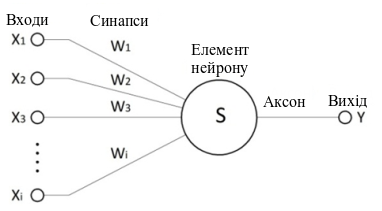
\includegraphics [width=.5\linewidth] {neuron}
	\caption{Загальний вигляд нейрона}
	\label{img:neuron}
\end{figure}

Кожна однонаправлена зв'язок характеризується вагою $w_i$ (величиною синаптичного зв'язку), який за фізичному змісту еквівалентен до електричної провідності. Додатні та відʼємні значення $w_i$ відповідають збудженому або загальмованому стану синапсів. Сума всіх входів визначає поточний стан нейрона \cite{Чураков_2014}

\begin{equation}
\label{eq:equation12}
s=\sum_{i=1}^n x_i w_i.
\end{equation}

Вихід нейрона є функція його стану:

\begin{equation}
\label{eq:equation13}
y=f(s).
\end{equation}

При використанні НМ в задачі розпізнавання мовних сигналах необхідно побудувати відповідну певну для цього завдання мережу, далі навчити її множині мовних сигналів --- підібрати вагові коефіцієнти синапсів для досягнення мінімізації кількості помилок.

\subsection{Аналіз з використанням прихованих марковських моделей}

Одним з найбільш ефективних методів обробки (розпізнавання) мовних сигналів є метод з використанням ПММ. ПММ - статистична модель, що імітує роботу процесу, схожого на марковский процес з невідомими параметрами. Головним завданням СММ є визначення (розгадування) невідомих параметрів на основі спостережуваних. Отримані параметри можуть бути використані в подальшому аналізі, наприклад, для розпізнавання образів.

Застосування ПММ в розпізнаванні грунтується на наступних припущеннях \cite{Огнев_2013}:

\begin{itemize}
	\item мовний сигнал може бути сегментований на фрагменти (стани), всередині яких сигнал може розглядатися як стаціонарний. Перехід між цими станами здійснюється миттєво;
	\item ймовірність появи символу, що породжується моделлю, залежить тільки від поточного стану моделі і не залежить від попередніх породжених символів.
\end{itemize}

Існує кілька типів ПММ, що розрізняються за своєю топологією. Детально топології ПММ розглянуті в \cite{Моттль_1999}.

Для прикладу на рис. \ref{img:hmm} представлена топологія подібної ПММ з трьома станами. ПММ є кінцевий автомат, що змінює свій стан в кожен дискретний момент часу $n$. Перехід зі стану $S_i$ в стан $S_j$ здійснюється випадковим чином з ймовірністю $a_{ij}$. У кожен дискретний момент часу модель породжує вектор спостережень $O_n$ з ймовірністю $b_j(O_n)$.

\begin{figure}
	\centering
	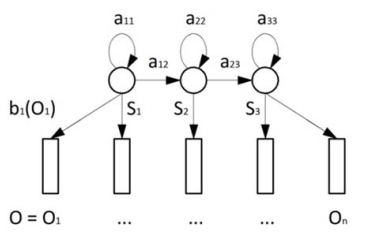
\includegraphics [width=.5\linewidth] {hmm}
	\caption{Топологія ПММ з трьома станами}
	\label{img:hmm}
\end{figure}

\subsection{Аналіз з використанням динамічного трансформування часу}

Відомо, що мовний сигнал швидко змінюється в часі. Різні вимови одного і того ж слова зазвичай мають різну тривалість, а вимови одного і того ж слова однаковою тривалості відрізняються в середині через різні частини слова, які вимовляються з різною швидкістю. Щоб отримати оцінку розбіжності між двома мовними сигналами, представленими як вектори, має бути виконано вирівнювання за часом, який можна реалізувати за допомогою ДТВ \cite{Goldenstein_2013}.

ДТВ є методом еластичного порівняння вектора спостережень з шаблоном, що зберігається. Вектор спостережень і шаблон лежать на відповідних осях сітки (рис. \ref{img:dtt}). Для кожного осередку сітки вираховується різниця між відповідними фрагментами вектора спостережень і шаблону. Оптимальне вирівнювання між вектором спостережень і шаблоном показано маршрутом, що проходить по сітці.

\begin{figure}
	\centering
	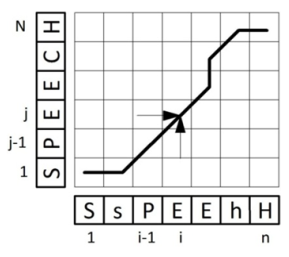
\includegraphics [width=.5\linewidth] {dtt}
	\caption{Робота методу динамічного програмування}
	\label{img:dtt}
\end{figure}

Метод ДТЧ працює з фрагментами, тобто аналіз ознак складається з обробки вектора ознак в регулярних інтервалах. Так як вектор ознак може мати безліч фрагментів, потрібні засоби розрахунку локальної оцінки відстані. Оцінка відстані між двома векторами ознак розраховується за допомогою Евклідової відстані

\begin{equation}
\label{eq:equation14}
d(x,y)=\sqrt{\sum_i(x_i-y_i)^2},
\end{equation}

\noindent
де $x_i$, $y_i$ --- порівнювані фрагменти; $i$ --- номер фрагменту.

Хоча обчислення Евклідової відстані в обчислювальному відношенні не вигідно в порівнянні з будь-якою іншою операцією, воно дає найкращі результати для розпізнавання.

На малюнку шаблон показаний вертикально, а спостережуваний сигнал --- горизонтально. Вхідний сигнал «SsPEEhH» --- це зашумлена версія шаблону «SPEECH». Ідея методу полягає в тому, що «h» --- це найближче збіг з «H» в порівнянні з чимось ще в шаблоні. Вхідний сигнал «SsPEEhH» порівнюється з усіма шаблонами, що зберігаються в словнику. Результатом порівняння буде шаблон, для якого було знайдено мінімальне розходження між вхідним сигналом і шаблоном. Глобальна оцінка розбіжності для маршруту --- це просто сума локальних відстаней між фрагментами сигналу і шаблону \cite{Алимурадов_2015}.

\subsection{Недоліки традиційних систем розпізнання мови}
Сучасні системи розпізнання мови в більшій своїй частині засновані на статистичних методах, використовують потужній апарат теорії ймовірностей та математичної статистики, що дає змогу суттєво підвищити якість розпізнання. Основні методи розпізнання мови --- це приховані Марківські моделі та штучні нейронні мережі \cite{Makovkin_2006, Gefke_2012}. Але у сучасних системах більш поширеними є моделі на нейронних мережах, оскільки вони мають більшу швидкодію та стійкість до шумів \cite{Hinton_2012}.

Звісно, на вхід до нейронної мережі не подають «сирий» звук — амплітуду коливань по часу, адже це не дуже інформативна форма представлення акустичного сигналу для аналізу. Більш інформативним є спектр сигналу, але на практиці найчастіше використовується мел-перетворення, в якому звуковий сигнал нарізується на фрейми розміром 20–40 мс, спектр кожного з яких масштабується через банк фільтрів та логарифмується для отримання даних, найбільш наближених до людського сприйняття \cite{Saini_2013}.

Існує досить багато таких систем і вони доволі якісно виконують свою задачу. Але в більшості своїй ці системи розраховані на роботу в приміщеннях без сильних шумів, залучення дикторів з чіткою вимовою та використання потужних комп’ютерів або віддалених серверів, як, наприклад, Google Voice Search. Та й ці системи неідеальні, в них не вирішені проблеми фільтрації шумів та розпізнання великих об’ємів даних, обмежені можливості налаштування під різні умови та різних дикторів \cite{Volkov_2014}. Так, наприклад, в системах мовного управління бортовим обладнанням літаків мінімальна можлива якість становить 95\%, а час розпізнавання не повинен перевищувати 0,2 с при темпі мовлення порядку 100 слів за хвилину \cite{Bondaros_2007}. Навіть у рамках однієї системи розпізнавання ці параметри можуть змінюватися в залежності від багатьох факторів, у тому числі таких, що визначаються умовами польоту, різними акустичними перешкодами, впливом пілотажних перевантажень тощо. \cite{Korsun_2013}.

Фактично, ті досягнення, які сьогодні здобуті в традиційних системах розпізнання мови, вже можуть бути використані для забезпечення голосової взаємодії в управлінні дистрибуцією. Проте вони не в змозі повністю забезпечити автоматизацію голосової взаємодії в задачах управління дистрибуцією, оскільки немає можливості а ні встановити у кабіні водія потужне обладнання, а ні забезпечити стабільний та швидкісний доступ до інтернету. Крім того, кабіна водія — це неконтрольоване акустичне середовище з високим рівнем шуму. Проблема багатодикторності також актуальна для дистрибуції, адже у таких компаніях зазвичай працює від декількох десятків до кількох сотень і навіть тисяч водіїв, в яких можуть буди дефекти вимови, різноманітні акценти та інші індивідуальні особливості мовлення.

\section{Новітні підходи до автоматизації голосової взаємодії} \label{sect1_5}

Японський дослідник з університету Осаки Ішігуро Хіроші з колегами вивчали різні аспекти комунікації та інформаційно-комунікаційних технологій, як, наприклад, використання комунікації з людиноподібними роботами в якості терапевтичної дії для людей похилого віку \cite{Nishio_2015}, аутистів \cite{Kumazaki_2016} чи просто замкнутих у собі людей, педагогічної дії щодо дітей та немовлят \cite{Park_2015} тощо. Зокрема він проводив дослідження голосової комунікації двох людей опосередковано через комп’ютер \cite{Ishiguro_2016}. 

У цьому дослідженні пара спілкувалася на загальні теми, обираючи варіанти своєї репліки із заздалегідь написаного дерева варіантів, свого роду сценарію. Жодному з партнерів не потрібно було нічого промовляти вголос: людині надавався набір з варіантів реплік на вибір, потрібно було лише натиснути на ту з них, яку б вона хотіла  промовити, і ця репліка лунала з динаміків. У залежності від використаної репліки програма вибирала з дерева сценаріїв можливі варіанти відповідей і надавала їх на вибір співрозмовнику. Співрозмовник у свою чергу, чуючи репліку першої людини, обирав свою з наданих варіантів. Це дослідження було спрямоване на подолання сором’язливості при спілкуванні з особами протилежної статі (що є особливо актуальним для Японії). Але такий підхід заздалегідь написаного дерева сценаріїв комунікації можна використовувати і в інших сферах.

У доповіді на світовому психологічному конгресі 2016 проф. Ішігуро демонстрував використання цього сценарного підходу для роботів на виставках та в музеях. Що б уникнути необхідності розпізнавання голосу в шумному середовищі, поряд з експонатом ставиться людиноподібний робот та монітор, на якому показані варіанти запитань. Натискаючи на різні репліки, відвідувач може спілкуватися з роботом по заздалегідь написаному дереву сценаріїв, розпитуючи його про експонат, а робот буде відповідати голосом.

На жаль для управління дистрибуцією постає зворотне завдання — водій має повідомити певну інформацію в систему і при цьому не повинен відволікатися на натискання кнопок на екрані. Тому пряме використання такої технології неможливе. Але застосування підходу описання всіх можливих сценаріїв комунікації в залежності від контексту дозволить знизити кількість інформації, яку треба розпізнати, а отже і підвищити якість.

Наразi існує новий підхід до голосового управління, заснований на теорії несилової взаємодії \cite{Teslia_2010} — рефлекторна система голосового управління \cite{Egorchenkov_2016}. Ідея, покладена в основу цього підходу, полягає в тому, щоб замість переведення голосової інформації в текстову репрезентацію, аналізувати безпосередньо інформаційну складову сказаного, визначаючи, яку з відомих реакцій потрібно виконати. «Традиційні системи розпізнання мови засновані на принципі: „усна мова“ → „репрезентація мови набором лінгвістичних конструкцій“ → „розуміння мови“. На основі теорії несиловой взаємодій може бути запропонована інша модель розпізнання природної мови: „усна мова“ → „розрахунок несилової (інформаційної) взаємодії на реакції“ → „реакція (розуміння чи поведінка)“» \cite{Teslia_2014}.

Така модель розпізнання називається рефлекторною, оскільки побудована за аналогією зі структурою умовного рефлексу, в якому виділяються афектори, центральний компонент та ефектори. Така модель може бути добре поєднана з ідеєю використання дерева сценаріїв, оскільки сценарії також складаються із реакцій, і одиницею моделювання стає не лінгвістична особливість мовлення, а реакція (або команда), яка може бути врахована автоматизованою системою розраховування маршрутів. Тобто, суть цього підходу полягає в тому, щоб перейти до іншої одиниці розпізнання мови. У психології дискурсивного мислення і рефлексивній психології також накопичено досвід аналізу мови, через виокремлення інших одиниць — функціональних висловлювань \cite{Naydonov_2008}.

Оскільки в такій системі не потрібні словники, складні інтелектуальні моделі аналізу тексту та граматики, вони мають низку переваг порівняно з традиційними системами: багатодикторність, варіабельність природної мови, можливість обробки команд офлайн прямо на пристрої, робота в умовах шумів (неконтрольованого акустично середовища), простота алгоритмів та менша складність і ціна реалізації \cite{Teslia_2013}.

У загальному випадку система рефлекторного голосового управління складається з трьох компонентів:

1. \textit{Фонемний стенограф}

Відповідає за перетворення відцифрованого вхідного звукового сигналу, що поміщає усну мову в набір фонем або слів.

2. \textit{Ядро системи}

Здійснює моделювання системи голосового управління. Містить програмну реалізацію всіх моделей, методів та алгоритмів системи, набір команд, протокол роботи, налаштування тощо.

3. \textit{База даних розпізнання мови з можливістю навчання}

Забезпечує зберігання інформаційної бази розпізнання мови та виділення керуючого впливу. У базі даних зберігається статистика вхідних впливів та відповідних їм вихідних реакцій системи.

Варто зазначити, що модуль фонемного стенографа може бути забезпечений різними програмними засобами, що робить систему гнучкішою та більш адаптивною до умов середовища. Єгорченков \cite{Egorchenkov_2016} наводить перелік можливих модулів фонемного стенографа. Провівши порівняльне зіставлення стенографів з цього переліку, можна стверджувати, що найбільш прийнятним для задач дистрибуції є фонетичний стенограф на основі Julius speech recognition tool \cite{Pylypenko_2009}, оскільки він у своїй роботі не потребує ні доступу до інтернету, ні великих словникових баз, а дає на виході «сирі» фонеми (наприклад, «п ъ й! А м а» для слова «Прямо»), які можуть навіть краще сприйматися рефлекторною системою для подальшого визначення інформаційного компоненту, ніж розпізнані слова, через вищу (в останньому випадку) ймовірність помилки.

\section{Постановка задачі дослідження} \label{sect1_6}

Виходячи з того, що \todo{...}, \textbf{наукова задача} дисертаційної роботи полягатиме в розробці моделей і методів інтеграції формалізації голосової інформації з управлінням процесом дистрибуції в єдиній системі формалізації голосової інформації в системах диспетчерського контролю за рухом автотранспорту.

У процесі вирішення наукової задачі висунута наступна \textbf{гіпотеза}: \todo{...}

\textbf{Основна ідея} даної наукової роботи полягає в тому, що вирішення поставленої наукової задачі можливо за рахунок:

\begin{itemize}
	\item \todo{...}
	\item \todo{...}
\end{itemize}

\textbf{Реалізація} цих ідей в рамках проведених досліджень може бути здійснена на підставі глибокого вивчення, виявлення сильних і слабких сторін методів та інструментів \todo{...}

\textbf{Предметною галузю дослідження} є \todo{...}.

\textbf{Дослідження}, результати яких викладені в подальших розділах цієї роботи, спрямовані:

\begin{itemize}
	\item на визначення методики досліджень і побудови \todo{науково-методологічних} основ автоматизації голосової взаємодії (розділ 2);
	\item на розробку методів формалізації голосової інформації в системах диспетчерського контролю за рухом автотранспорту (розділ 3);
	\item на створення засобів формалізації голосової інформації в системах диспетчерського контролю за рухом автотранспорту(розділ 4).
\end{itemize}

\section*{Висновки до розділу 1}
\addcontentsline{toc}{section}{Висновки до розділу 1}
